\documentclass[11pt,a4paper]{article}
\usepackage[T1]{fontenc}
\usepackage[utf8]{inputenc}
\usepackage{lmodern}
\usepackage{geometry}
\usepackage{graphicx}
\usepackage{booktabs}
\usepackage{tabularx}
\usepackage{array}
\usepackage{amsmath}
\usepackage{amssymb}
\usepackage{siunitx}
\usepackage{longtable}
\usepackage{float}
\usepackage{subcaption}
\usepackage{xcolor}
\usepackage{caption}
\usepackage{hyperref}
\geometry{margin=2.0cm}
\graphicspath{{figures/}}
\captionsetup{font=small,labelfont=bf}
\newcommand{\RMSE}{\ensuremath{\mathrm{RMSE}}}
\newcommand{\MAE}{\ensuremath{\mathrm{MAE}}}
\newcommand{\Czon}{\ensuremath{C_{\mathrm{zon}}}}
\newcommand{\Tsupply}{\ensuremath{T_{\mathrm{sup}}}}
\newcommand{\That}{\ensuremath{\widehat{T}}}
\renewcommand{\thetable}{S\arabic{table}}
\renewcommand{\thefigure}{S\arabic{figure}}
\title{Supplementary Material for\\[2pt]
\emph{The Fidelity--Utility Paradox in Surrogate-Based
Reinforcement Learning for HVAC Control}}
\author{}
\date{}

\begin{document}
\maketitle

\noindent This document is the Supplementary Material for the above manuscript. It
provides the complete content-to-artefact provenance maps for the three evidence
blocks (Supplementary Tables~S1--S3) and the parameter, configuration, and
interface tables referenced from the main text (Supplementary Tables~S4--S9).
Every figure, table, and inline number in the main text can be traced through these
maps to the exact versioned source file in the project's \texttt{reports/} and
\texttt{outputs/} trees.

\renewcommand{\thetable}{S\arabic{table}}
\setcounter{table}{0}

\footnotesize
\begin{longtable}{@{}p{0.40\linewidth} p{0.52\linewidth}@{}}
\caption{Results~I content-to-artefact provenance map (rebuild: \texttt{python3 -B docs/results1\_digital\_twin\_overleaf/build\_results1\_overleaf.py}).}\label{tab:prov-r1}\\
\textbf{Content} & \textbf{Source artefact}\\ \midrule \endfirsthead
\textbf{Content} & \textbf{Source artefact}\\ \midrule \endhead
Data corpora table & \texttt{reports/\allowbreak hou\_\allowbreak evins\_\allowbreak sample\_\allowbreak generation\_\allowbreak table.csv} \\
v3 architecture / training hyperparameters & \texttt{reports/\allowbreak hou\_\allowbreak evins\_\allowbreak training\_\allowbreak hyperparams\_\allowbreak table.csv} \\
Feature scaling + physical-constraint table & \texttt{reports/\allowbreak hou\_\allowbreak evins\_\allowbreak scaling\_\allowbreak table.csv} \\
v3 learning curve + best-epoch / val R\textasciicircum{}2 & \texttt{outputs/\allowbreak surrogate\_\allowbreak v2/\allowbreak train\_\allowbreak history\_\allowbreak v2.csv} \\
Multi-horizon rollout RMSE and 24 h R\textasciicircum{}2 (S11) & \texttt{reports/\allowbreak hou\_\allowbreak evins\_\allowbreak predictive\_\allowbreak validity\_\allowbreak table.csv} \\
Stage A alignment, Stage B excitation, C\_zon & \texttt{outputs/\allowbreak surrogate\_\allowbreak v35\_\allowbreak inverse\_\allowbreak boptest\_\allowbreak 15min\_\allowbreak episodeaware/\allowbreak calibration\_\allowbreak summary\_\allowbreak boptest\_\allowbreak v35.json} \\
Stage B C\_zon trajectory + stability band & \texttt{outputs/\allowbreak surrogate\_\allowbreak v35\_\allowbreak inverse\_\allowbreak boptest\_\allowbreak 15min\_\allowbreak episodeaware/\allowbreak stage\_\allowbreak b\_\allowbreak history\_\allowbreak v35.csv} \\
Canonical Stage C power head (power MAE 482 W) & \texttt{outputs/\allowbreak surrogate\_\allowbreak v35\_\allowbreak inverse\_\allowbreak boptest\_\allowbreak 15min\_\allowbreak power\_\allowbreak head\_\allowbreak only/\allowbreak calibration\_\allowbreak summary\_\allowbreak boptest\_\allowbreak v35.json} \\
Temperature rollout: 24 h RMSE, P95, residuals, & \texttt{outputs/\allowbreak surrogate\_\allowbreak v35\_\allowbreak rollout\_\allowbreak prepared\_\allowbreak 15min\_\allowbreak power\_\allowbreak head\_\allowbreak only/\allowbreak calibrated\_\allowbreak v35/\allowbreak  persistence baseline                                  (all\_\allowbreak full\_\allowbreak rollouts.csv, horizon\_\allowbreak metrics.csv, window\_\allowbreak errors.csv, episode\_\allowbreak summary.csv)} \\
Power-channel ASHRAE-G14 metrics (canonical) & \texttt{outputs/\allowbreak surrogate\_\allowbreak v35\_\allowbreak rollout\_\allowbreak prepared\_\allowbreak 15min\_\allowbreak power\_\allowbreak head\_\allowbreak only/\allowbreak calibrated\_\allowbreak v35/\allowbreak all\_\allowbreak full\_\allowbreak rollouts.csv} \\
v3 rollout reference & \texttt{outputs/\allowbreak surrogate\_\allowbreak v3\_\allowbreak rollout\_\allowbreak prepared\_\allowbreak 15min/\allowbreak v3/\allowbreak } \\
Matched-corpus four-variant + decomposition & \texttt{reports/\allowbreak block1\_\allowbreak corpus\_\allowbreak matched\_\allowbreak comparison.csv (+ .json)} \\
Runtime throughput (steps/s, median/P95 ms) & \texttt{reports/\allowbreak speed\_\allowbreak benchmark\_\allowbreak table.csv} \\
Figures rie\_fig01..08 (PDF + PNG) & \texttt{docs/\allowbreak results1\_\allowbreak digital\_\allowbreak twin\_\allowbreak overleaf/\allowbreak figures/\allowbreak   (generated)} \\
\bottomrule
\end{longtable}
\normalsize

\footnotesize
\begin{longtable}{@{}p{0.40\linewidth} p{0.52\linewidth}@{}}
\caption{Results~II content-to-artefact provenance map (rebuild: \texttt{python3 -B evaluation/run\_block2.py build-reports}).}\label{tab:prov-r2}\\
\textbf{Content} & \textbf{Source artefact}\\ \midrule \endfirsthead
\textbf{Content} & \textbf{Source artefact}\\ \midrule \endhead
Pure v3 thermostatic baseline KPIs & \texttt{outputs/\allowbreak bestest\_\allowbreak air\_\allowbreak article7\_\allowbreak style\_\allowbreak 15min/\allowbreak summary.csv} \\
Temporal-coarse-graining ablation (tab:coarse\_graining) & \texttt{reports/\allowbreak block2\_\allowbreak v3\_\allowbreak 15min\_\allowbreak closed\_\allowbreak loop\_\allowbreak comparison.csv ; outputs/\allowbreak bestest\_\allowbreak air\_\allowbreak pure\_\allowbreak v3\_\allowbreak 15min/\allowbreak summary.csv} \\
Direct-v3.5 warm-start negative control & \texttt{outputs/\allowbreak block2\_\allowbreak thermostatic\_\allowbreak warmstart\_\allowbreak utility/\allowbreak comparison\_\allowbreak summary.csv} \\
Thermostatic hybrid sweep (canonical hybrid\_l010) & \texttt{outputs/\allowbreak block2\_\allowbreak thermostatic\_\allowbreak *hybrid*/\allowbreak   (benchmark summaries)} \\
Architecture justification on live BOPTEST (S9) & \texttt{reports/\allowbreak hou\_\allowbreak evins\_\allowbreak architecture\_\allowbreak justification\_\allowbreak table.csv} \\
Fidelity-to-RL transfer-gap diagnostics & \texttt{reports/\allowbreak hybrid\_\allowbreak transfer\_\allowbreak comparison.csv (+ reports/\allowbreak figures/\allowbreak hybrid\_\allowbreak transfer\_\allowbreak gap\_\allowbreak comparison.png)} \\
HDRL sweep (best lambda\_temp = 0.00) & \texttt{outputs/\allowbreak block2\_\allowbreak hdrl\_\allowbreak hybrid\_\allowbreak v3\_\allowbreak v35\_\allowbreak l0\{00,03,05,10\}/\allowbreak } \\
MORL 5D vs 17D observation-interface ablation & \texttt{reports/\allowbreak block2\_\allowbreak morl\_\allowbreak 5d\_\allowbreak reconstructed\_\allowbreak comparison.csv} \\
MORL single-seed Pareto sweep & \texttt{outputs/\allowbreak morl\_\allowbreak pareto\_\allowbreak hybrid\_\allowbreak power\_\allowbreak only/\allowbreak <tag>/\allowbreak  ; reports/\allowbreak morl\_\allowbreak pareto\_\allowbreak front\_\allowbreak table.csv} \\
MORL N=5 canonical seed variance & \texttt{reports/\allowbreak morl\_\allowbreak *canonical*.csv} \\
PI yearly baseline & \texttt{evaluation/\allowbreak run\_\allowbreak block2.py pi-yearly  (m\_\allowbreak s, violation, energy, RMSE\_\allowbreak T)} \\
Block 2 tables/figures rebuild & \texttt{evaluation/\allowbreak run\_\allowbreak block2.py build-reports  (Section 11)} \\
m\_s metric definition (r\_time + r\_sev) & \texttt{evaluation/\allowbreak benchmark\_\allowbreak bestest\_\allowbreak air\_\allowbreak article7\_\allowbreak style.py (compute\_\allowbreak safety\_\allowbreak metrics)} \\
Reward / action / comfort-band parameters & \texttt{configs/\allowbreak env.yaml  (morl + comfort\_\allowbreak shaping + action\_\allowbreak wrappers)} \\
17D observation feature groups & \texttt{envs/\allowbreak tsup\_\allowbreak features.py  (obs\_\allowbreak mode = extended)} \\
Targeted + yearly scenario definitions & \texttt{outputs/\allowbreak block2\_\allowbreak */\allowbreak scenario\_\allowbreak manifest.json} \\
Hybrid v3-vs-v3.5 disagreement statistics & \texttt{reports/\allowbreak hybrid\_\allowbreak disagreement\_\allowbreak summary.csv  (overall row)} \\
\bottomrule
\end{longtable}
\normalsize

\footnotesize
\begin{longtable}{@{}p{0.40\linewidth} p{0.52\linewidth}@{}}
\caption{Results~III content-to-artefact provenance map (rebuild: \texttt{Block~3 evaluation scripts (see manifests below)}).}\label{tab:prov-r3}\\
\textbf{Content} & \textbf{Source artefact}\\ \midrule \endfirsthead
\textbf{Content} & \textbf{Source artefact}\\ \midrule \endhead
Headline transfer matrix (m\_s, threshold, RMSE, C\_zon) & \texttt{reports/\allowbreak block3\_\allowbreak transfer\_\allowbreak matrix.csv} \\
Primary per-regime detail (none/partial/full) & \texttt{reports/\allowbreak block3\_\allowbreak bestest\_\allowbreak hydronic\_\allowbreak heat\_\allowbreak pump\_\allowbreak transfer\_\allowbreak summary.csv} \\
Secondary / stretch per-regime detail & \texttt{reports/\allowbreak block3\_\allowbreak bestest\_\allowbreak hydronic\_\allowbreak transfer\_\allowbreak summary.csv ; reports/\allowbreak block3\_\allowbreak singlezone\_\allowbreak commercial\_\allowbreak hydronic\_\allowbreak transfer\_\allowbreak summary.csv} \\
N=2 hydronic-family roll-up & \texttt{reports/\allowbreak block3\_\allowbreak hydronic\_\allowbreak family\_\allowbreak n2\_\allowbreak summary.csv} \\
C\_zon ratios + hydronic-family mean/std & \texttt{reports/\allowbreak block3\_\allowbreak transfer\_\allowbreak matrix.csv (c\_\allowbreak zon\_\allowbreak ratio\_\allowbreak vs\_\allowbreak bestest\_\allowbreak air); baseline 4.413e5 J/\allowbreak K (Block 1)} \\
Testcases / adapters / regimes / hypotheses / predictions & \texttt{configs/\allowbreak block3\_\allowbreak testcase\_\allowbreak manifest.yaml ; configs/\allowbreak block3\_\allowbreak actuator\_\allowbreak mapping\_\allowbreak *.yaml} \\
Audit anchors & \texttt{git log: 1861e48, 2f9d596, eb7091e, 46fbaa9, 645626e, 7ada793, cb7025f} \\
Figures (protocol, heatmap, RMSE gain, C\_zon, closure) & \texttt{docs/\allowbreak results3\_\allowbreak transferability\_\allowbreak overleaf/\allowbreak figures/\allowbreak   (Block 3 evaluation scripts)} \\
\bottomrule
\end{longtable}
\normalsize

\subsection*{Supplementary figures and tables}

The following figures and tables provide supporting schematics, calibration and controller diagnostics, and detailed per-regime and per-seed breakdowns. They are cited from Results~I--III (as Figure~S/Table~S references) but are not required to follow the main argument.

\begin{figure}[pos={!ht}]
  \centering
  \includegraphics[width=\linewidth]{\detokenize{rie_fig01_block1_artifact_chain.pdf}}
  \caption{Roadmap-derived Block 1 artifact chain. The figure reports the actual row counts, 24 h rollout errors, identified physical parameter, and speed benchmark values used to close Results I.}
  \label{fig:block1-chain}

{\footnotesize\itshape Schematic; not derived from a dataset.}
\end{figure}

\begin{figure}[pos={!ht}]
  \centering
  \includegraphics[width=\linewidth]{\detokenize{rie_fig02_surrogate_design.pdf}}
  \caption{Surrogate role separation inside Block 1. v3 is the compact dual-head rollout model; v3.5 adds Stage A/B/C physical identification and residual-head calibration.}
  \label{fig:surrogate-design}

{\footnotesize\itshape Schematic; not derived from a dataset.}
\end{figure}

\begin{figure}[pos={!ht}]
  \centering
  \includegraphics[width=0.78\linewidth]{\detokenize{rie_fig08_v3_learning_curve.pdf}}
  \caption{v3 supervised train/validation learning curves. Early stopping at the best validation epoch precedes any validation-loss upturn, indicating no overfitting at the selected checkpoint.}
  \label{fig:v3-learning-curve}

{\footnotesize\itshape Data: \texttt{outputs/\allowbreak surrogate\_\allowbreak v2/\allowbreak train\_\allowbreak history\_\allowbreak v2.csv}}
\end{figure}

\begin{figure}[pos={!ht}]
  \centering
  \includegraphics[width=0.74\linewidth]{\detokenize{rie_fig09_physics_consistency.pdf}}
  \caption{Physical-consistency audit: predicted next-step zone temperature versus the supply-temperature command for representative initial states. The response is monotone increasing, so the learned dynamics respect the correct sign of the control.}
  \label{fig:physics}

{\footnotesize\itshape Data: \texttt{outputs/\allowbreak surrogate\_\allowbreak v35\_\allowbreak rollout\_\allowbreak prepared\_\allowbreak 15min\_\allowbreak power\_\allowbreak head\_\allowbreak only/\allowbreak calibrated\_\allowbreak v35/\allowbreak all\_\allowbreak full\_\allowbreak rollouts.csv}}
\end{figure}

\begin{figure}[pos={!ht}]
  \centering
  \includegraphics[width=\linewidth]{\detokenize{rie_fig04_predictive_validity.pdf}}
  \caption{Predictive-validity diagnostics from prepared BOPTEST rollouts. Confidence bands are bootstrapped from real window-level errors, and the CDF reports engineering error tolerances at 0.5, 1.0, and 1.5~$^\circ$C.}
  \label{fig:predictive-validity}

{\footnotesize\itshape Data: \texttt{outputs/\allowbreak surrogate\_\allowbreak v35\_\allowbreak rollout\_\allowbreak prepared\_\allowbreak 15min\_\allowbreak episodeaware/\allowbreak calibrated\_\allowbreak v35/\allowbreak window\_\allowbreak errors.csv}}
\end{figure}

\begin{figure}[pos={!ht}]
  \centering
  \includegraphics[width=\linewidth]{\detokenize{rie_fig07_episode_replicability.pdf}}
  \caption{Replicative validity across the eight held-out BOPTEST episodes used by the Block 1 prepared-rollout artifacts. The dashed line marks a 1~$^\circ$C engineering reference.}
  \label{fig:episode-replicability}

{\footnotesize\itshape Data: \texttt{outputs/\allowbreak surrogate\_\allowbreak v35\_\allowbreak rollout\_\allowbreak prepared\_\allowbreak 15min\_\allowbreak episodeaware/\allowbreak calibrated\_\allowbreak v35/\allowbreak episode\_\allowbreak summary.csv}}
\end{figure}

\begin{table}[pos={!ht}]
\centering
\small
\caption{v3 configuration from the active model class and Hou-and-Evins reporting artifacts.}
\label{tab:v3-config}
\begin{tabularx}{0.86\linewidth}{lX}
\toprule
Item & Value \\
\midrule
Input dimension & 8 \\
Temperature head & HeatFlowNetV2, 7,105 params \\
Power head & PowerNetV2, 1,377 params \\
Total parameters & 8,482 \\
Epoch budget & 500 \\
Batch size & 256 \\
Learning rate & 1e-3 \\
Optimizer & AdamW \\
Early stopping & patience=30; improvement\_threshold=1e-6 \\
\bottomrule
\end{tabularx}
\end{table}

\begin{table}[pos={!ht}]
\centering
\scriptsize
\caption{Feature scaling and physical constraints used by the Block 1 surrogate interface.}
\label{tab:v3-scaling}
\begin{tabularx}{\linewidth}{lXXX}
\toprule
Variable & Scaling method & Parameters & Engineering role \\
\midrule
surrogate\_t\_zone & affine min-max to [-1, 1] & min=15 C; max=35 C & Keeps the learned thermal state within the training support used by the direct-TSup surrogate. \\
surrogate\_t\_amb & affine min-max to [-1, 1] & min=-10 C; max=40 C & Normalizes outdoor-air temperature for the heat and power heads. \\
hour & cyclic sine/cosine & sin(2*pi*hour/24); cos(2*pi*hour/24) & Avoids discontinuity between hour 23 and hour 0. \\
day & cyclic sine/cosine & sin(2*pi*day/365); cos(2*pi*day/365) & Represents seasonal phase without an artificial year-end jump. \\
a0\_raw & native action domain & [-1, 1] maps to 18..35 C supply temperature & Preserves the PPO action coordinate while keeping physical supply-temperature bounds explicit. \\
a1\_raw & native action domain & [-1, 1] maps to 0..1 fan command & Keeps fan modulation aligned with the controller action range. \\
power\_head\_output & Softplus multiplied by P\_MAX & P\_MAX=5500 W & Guarantees non-negative predicted HVAC power. \\
\bottomrule
\end{tabularx}
\end{table}

\begin{table}[pos={!ht}]
\centering
\small
\caption{Stage A telemetry-alignment operations from the calibration-summary JSON.}
\label{tab:stage-a}
\begin{tabularx}{\linewidth}{llX}
\toprule
Operation & Estimated value & Effect \\
\midrule
Latency compensation & 1 step (15 min) & latency-search RMSE 0.378 C \\
Temperature bias removal & -0.1049 C & median residual offset \\
Power affine normalization & scale -0.702, bias 1148 W & global power-channel rescale \\
Post-Stage-A temperature RMSE & 0.2383 C & baseline for Stage B \\
Post-Stage-A power MAE & 514.4 W & baseline for Stage C \\
\bottomrule
\end{tabularx}
\end{table}

\begin{table}[pos={!ht}]
\centering
\small
\caption{Stage B excitation filtering and physical identification of \(\Czon\).}
\label{tab:stage-b}
\begin{tabularx}{\linewidth}{llX}
\toprule
Parameter & Value & Notes \\
\midrule
C\_zon prior & $4.200\times10^5$ J/K & air volume x specific heat \\
C\_zon after Stage B & $4.413\times10^5$ J/K & +5.1\% vs prior \\
Stage B epochs & 120 & episode-aware run \\
C\_zon learning rate & $10^{-3}$ & dedicated scalar LR \\
Excitation quantile & 0.95 & |dT| threshold 0.1759 \\
Excitation rows & 403 / 8058 & mean score 0.240 vs 0.069 \\
\bottomrule
\end{tabularx}
\end{table}

\begin{figure}[pos={!ht}]
  \centering
  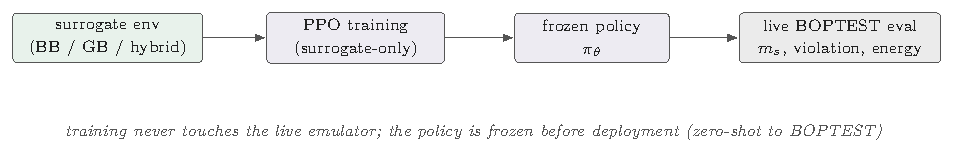
\includegraphics[width=0.94\linewidth]{fig_block2_pipeline.pdf}
  \caption{Block 2 controller-learning pipeline. The experiments separate the rollout model, the physical regularizer, the controller family, the observation interface, and live BOPTEST validation.}
  \label{fig:block2_pipeline}

{\footnotesize\itshape Schematic; not derived from a dataset.}
\end{figure}

\begin{figure}[pos={!ht}]
  \centering
  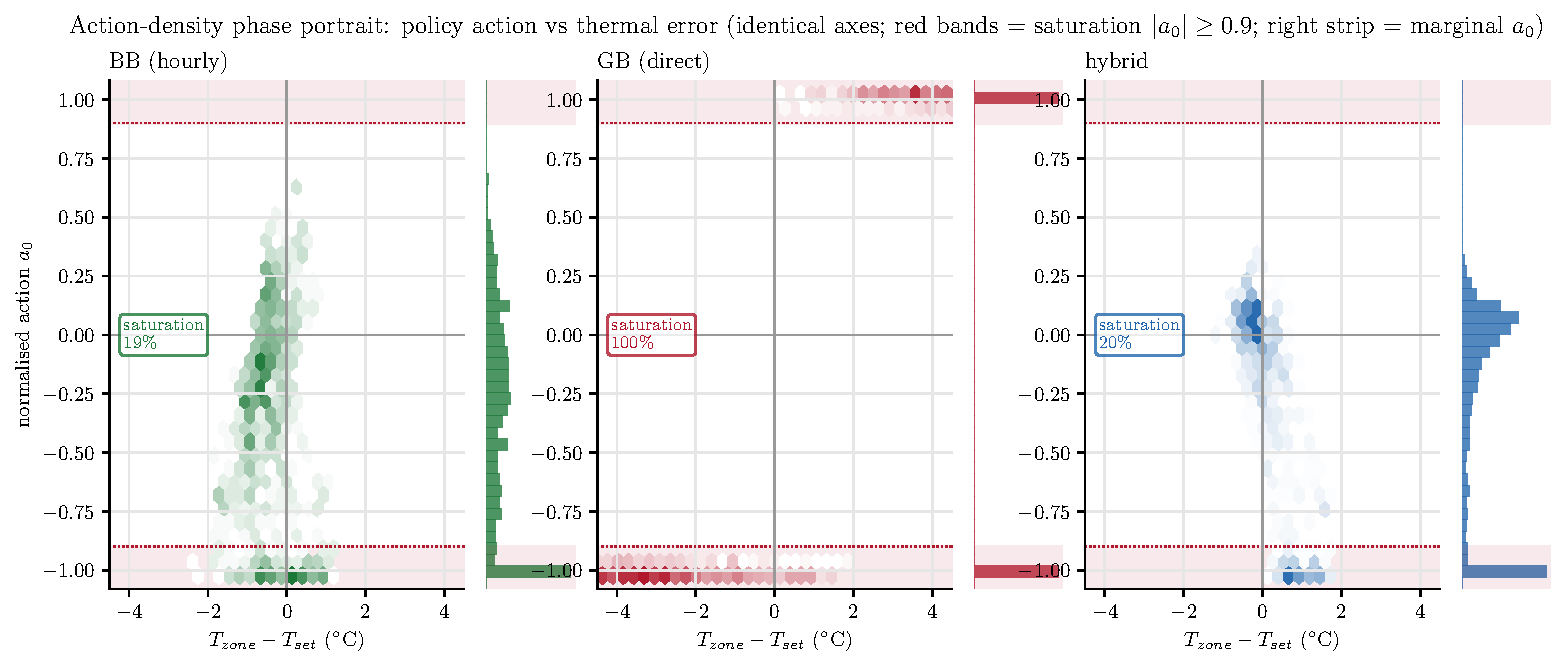
\includegraphics[width=0.96\linewidth]{block2_q1_polish_phase_density.pdf}
  \caption{Phase portrait as empirical state-action density. The saturation bands near $a_0=\pm1$ expose the bang-bang behavior of direct v3.5 PPO.}
  \label{fig:action_phase}

{\footnotesize\itshape Data: \texttt{outputs/\allowbreak block2\_\allowbreak thermostatic\_\allowbreak hybrid\_\allowbreak v3\_\allowbreak v35\_\allowbreak l010/\allowbreak }}
\end{figure}

\begin{figure}[pos={!ht}]
  \centering
  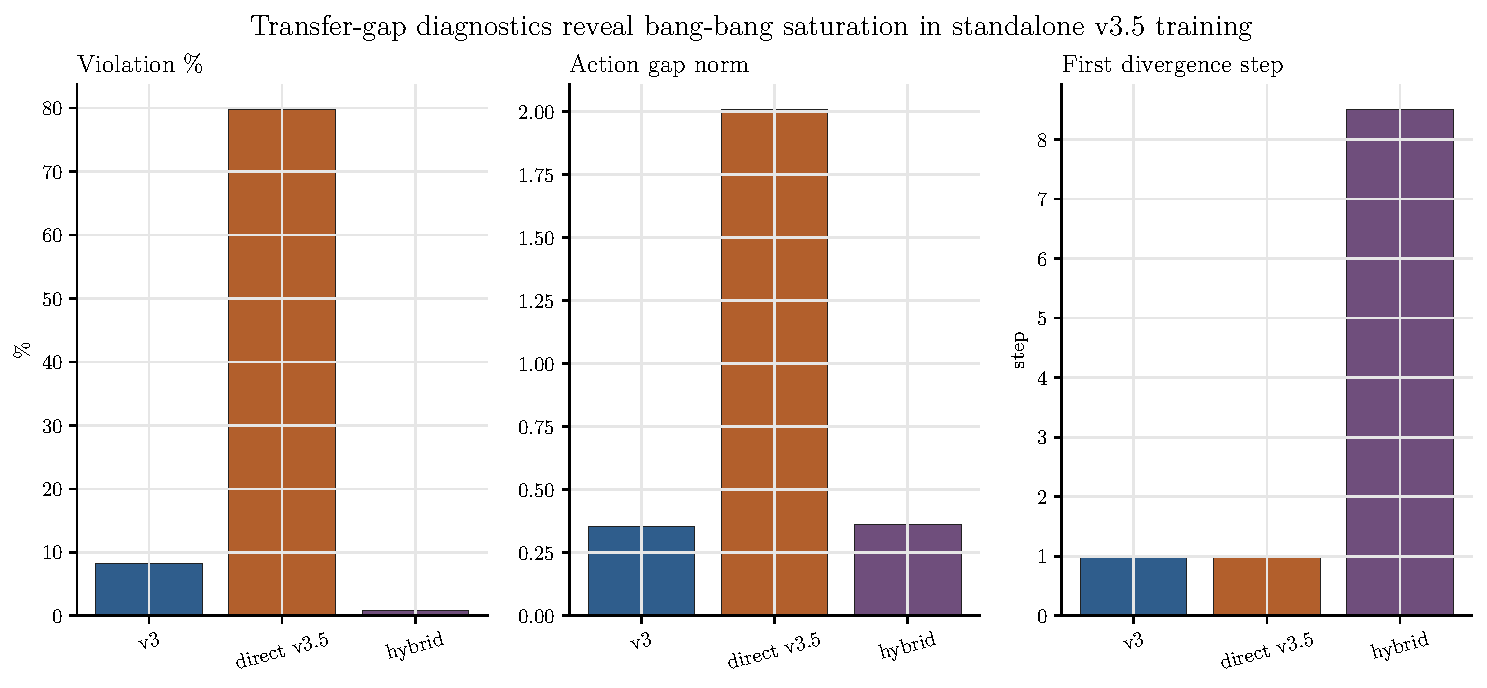
\includegraphics[width=0.86\linewidth]{block1_q1_fig10_transfer_gap_diagnostics.pdf}
  \caption{Transfer-gap diagnostics. Direct v3.5 has high action-gap norm and live-surrogate mismatch; the hybrid backend suppresses both.}
  \label{fig:transfer_gap}

{\footnotesize\itshape Data: \texttt{reports/\allowbreak hybrid\_\allowbreak transfer\_\allowbreak comparison.csv}}
\end{figure}

\begin{figure}[pos={!ht}]
  \centering
  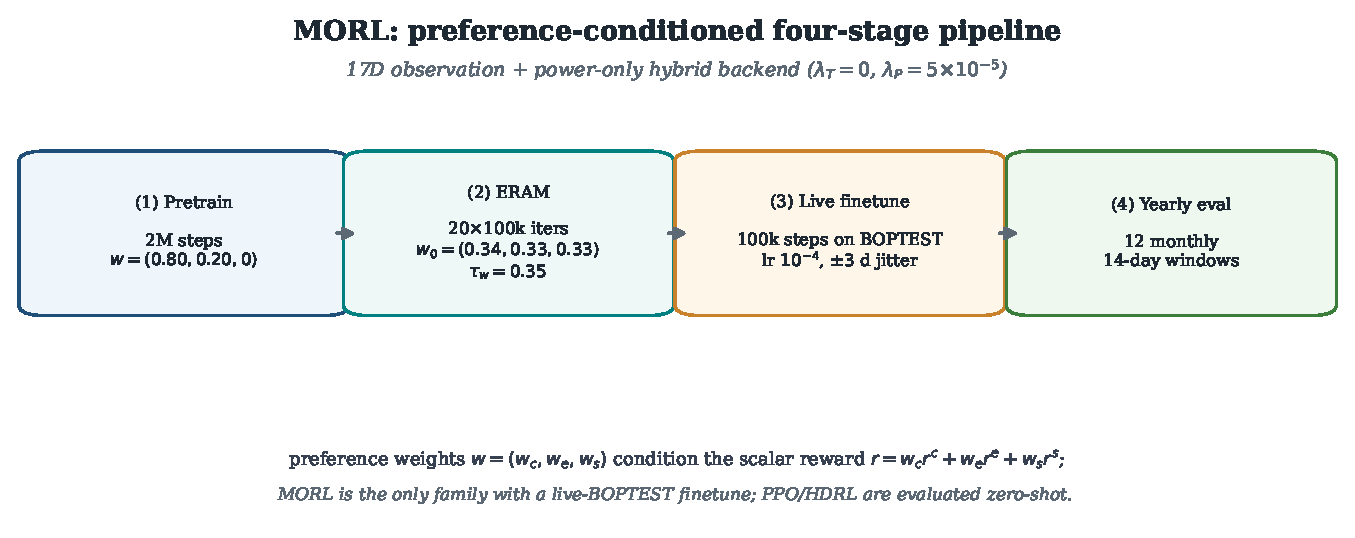
\includegraphics[width=0.98\linewidth]{fig_block2_morl_pipeline.pdf}
  \caption{MORL four-stage pipeline: surrogate pretrain $\to$ ERAM preference adaptation $\to$ live-BOPTEST finetune $\to$ yearly evaluation, all on the 17D power-only hybrid backend. The preference vector conditions the scalarized reward.}
  \label{fig:morl_pipeline}

{\footnotesize\itshape Schematic; not derived from a dataset.}
\end{figure}

\begin{figure}[pos={!ht}]
  \centering
  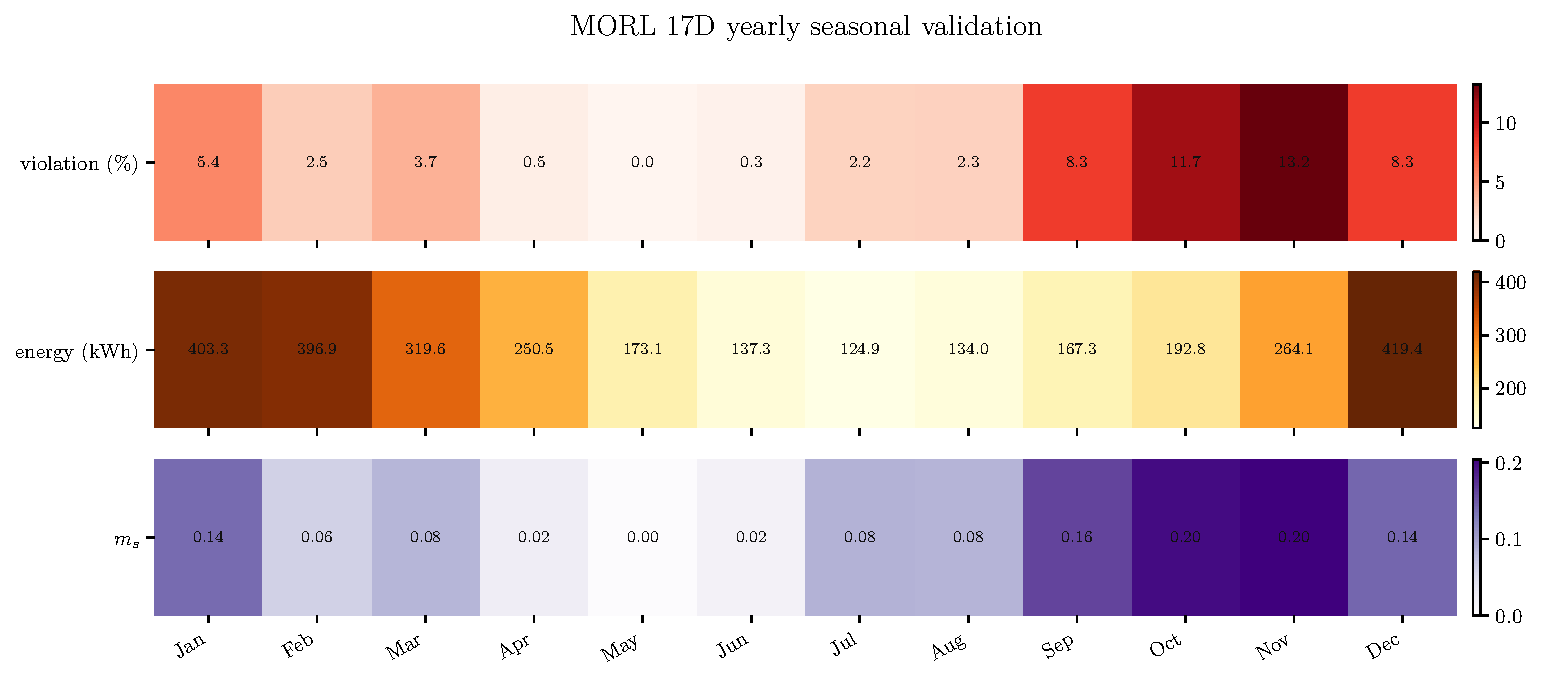
\includegraphics[width=0.88\linewidth]{block2_morl_17d_seasonal_heatmap.pdf}
  \caption{MORL seasonal performance heatmap under the 17D interface. The figure shows monthly structure but does not support the N=3 mechanism claim after N=5 extension.}
  \label{fig:morl_heatmap}

{\footnotesize\itshape Data: \texttt{reports/\allowbreak morl\_\allowbreak canonical\_\allowbreak seedfix\_\allowbreak yearly\_\allowbreak summary.csv}}
\end{figure}

\begin{figure}[pos={!ht}]
  \centering
  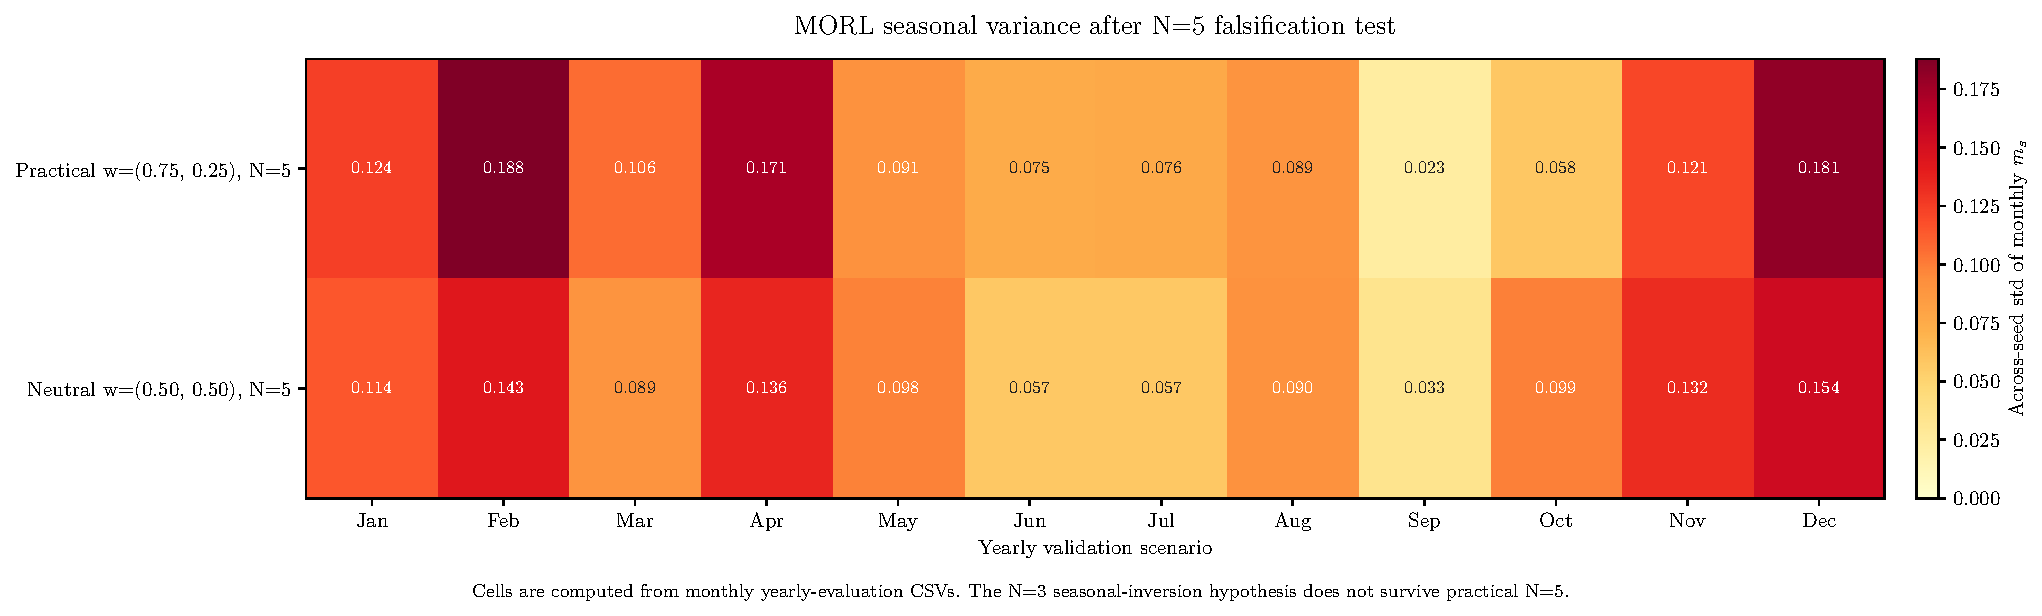
\includegraphics[width=0.88\linewidth]{block2_morl_seasonal_variance_inversion.pdf}
  \caption{Post-N=5 seasonal variance diagnostic. The earlier seasonal-inversion hypothesis is reported as falsified, not retained as a positive mechanism claim.}
  \label{fig:seasonal_falsification}

{\footnotesize\itshape Data: \texttt{reports/\allowbreak morl\_\allowbreak canonical\_\allowbreak seedfix\_\allowbreak yearly\_\allowbreak per\_\allowbreak seed.csv}}
\end{figure}

\begin{table}[pos={!ht}]
\centering
\caption{PPO training configuration used in Block 2 (verified from the project training scripts and configuration files).}
\label{tab:ppo_hparams}
\small
\begin{tabular}{lllll}
\toprule
Parameter & Thermostatic PPO & HDRL & MORL pretrain & MORL finetune \\
\midrule
Algorithm & PPO, MlpPolicy & PPO, MlpPolicy & PPO, MlpPolicy & PPO load+continue \\
Learning rate & $3.0{\times}10^{-4}$ & $3.0{\times}10^{-4}$ & $3.0{\times}10^{-4}$ & $1.0{\times}10^{-4}$ \\
\texttt{n\_steps} & 1024 & 1024 & 2048 & inherited \\
\texttt{batch\_size} & 4096 & 2048 & 64 & inherited \\
\texttt{n\_epochs} & 10 & 10 & 10 & 10 \\
$\gamma$ & 0.99 & 0.99 & 0.99 & 0.99 \\
GAE $\lambda$ & 0.95 & 0.95 & 0.95 & 0.95 \\
Clip range & 0.20 & 0.20 & 0.20 & 0.20 \\
Total timesteps & 10M & 12M & 2M & 100k \\
Seed & 42 & 42 & 42 & 42--46 (N=5) \\
\bottomrule
\end{tabular}
\end{table}

\begin{table}[pos={!ht}]
\centering
\caption{Extended 17D observation feature groups (verified from \texttt{envs/tsup\_features.py}).}
\label{tab:obs17}
\small
\begin{tabularx}{\linewidth}{llX}
\toprule
Feature group & Dim. & Contents \\
\midrule
Physical state (basic) & 5 & $T_{\mathrm{zone}}$, CO$_2$, clipped-log power, prev. $T_{\mathrm{sup}}$, $T_{\mathrm{amb}}$ \\
Cyclic time & 4 & hour and day sine/cosine encodings \\
Ambient forecast & 5 & $T_{\mathrm{amb}}$ at $+1,+3,+6,+12,+24$ h \\
Previous action & 2 & $(a_{T_{\mathrm{sup}}}, a_{\mathrm{fan}})$ from last step \\
Temperature delta & 1 & causal-smoothed $\Delta T_{\mathrm{zone}}$ \\
Total (extended) & 17 & obs\_mode = extended \\
\bottomrule
\end{tabularx}
\end{table}

\begin{table}[pos={!ht}]
\centering
\caption{Reward-shaping parameters (verified from \texttt{configs/env.yaml}).}
\label{tab:reward}
\small
\begin{tabularx}{\linewidth}{llX}
\toprule
Component & Value & Role \\
\midrule
Comfort band & 21.0 / 24.0 C & comfort interval (band\_low/high) \\
Comfort deadband & 0.50 C & soft margin around band edges \\
In-band bonus & 0.050/step & reward for staying inside the band \\
Undershoot / overshoot weight & 1.15 / 1.15 & generic violation penalties \\
Cold-ambient asymmetry & 1.60 (amb $<8.0$ C) & extra cold-undershoot penalty \\
Hot-ambient asymmetry & 1.80 (amb $>24.0$ C) & extra hot-overshoot penalty \\
Heating action bonus & 0.04 ($T_{\mathrm{sup}}\ge 29.0$ C) & anti-degenerate shaping \\
Cooling action bonus & 0.06 ($T_{\mathrm{sup}}\le 21.0$ C) & anti-degenerate shaping \\
MORL weights ($w_c/w_e/w_s$) & 0.80 / 0.20 / 0.00 & canonical scalarization \\
Energy scale & $2e-4$ (W$\to$reward) & energy-to-reward conversion \\
\bottomrule
\end{tabularx}
\end{table}

\begin{table}[pos={!ht}]
\centering
\caption{Thermostatic hybrid $\lambda_T$ sweep design (roadmap \S5; $\lambda_P=5\times10^{-5}$ throughout). The mid point is the retained canonical.}
\label{tab:hybrid_sweep}
\small
\begin{tabular}{lll}
\toprule
$\lambda_T$ & Tag & Role \\
\midrule
0.05 & hybrid\_l005 & weaker censor (sweep bracket) \\
0.10 & hybrid\_l010 & \textbf{canonical} (retained; $m_s=0.087$ peak, $0.041$ typical) \\
0.15 & hybrid\_l015 & stronger censor (sweep bracket) \\
\bottomrule
\end{tabular}
\end{table}

\begin{table}[pos={!ht}]
\centering
\caption{Direct-v3.5 warm-start utility (\texttt{outputs/block2\_thermostatic\_warmstart\_utility/comparison\_summary.csv}).}
\label{tab:warmstart}
\small
\begin{tabular}{llrr}
\toprule
Mode & Scenario & $m_s$ & Violation (\%) \\
\midrule
scratch (random init) & peak & 0.465 & 31.70 \\
scratch (random init) & typical & 0.578 & 45.54 \\
warm-start (from v3.5) & peak & 1.270 & 83.93 \\
warm-start (from v3.5) & typical & 1.289 & 86.83 \\
\bottomrule
\end{tabular}
\end{table}

\begin{table}[pos={!ht}]
\centering
\caption{Per-seed MORL yearly metrics for the two canonical weight pairs (data: roadmap Section 11.1).}
\label{tab:morl_per_seed}
\small
\begin{tabular}{lrrrrrr}
\toprule
Pair (c/e) & Seed & RMSE$_T$ & Within 1$^\circ$C (\%) & Violation (\%) & Energy (kWh) & $m_s$ \\
\midrule
50/50 & 42 & 0.939 & 74.9 & 12.92 & 2843.6 & 0.193 \\
50/50 & 43 & 0.769 & 82.9 & 6.77 & 2872.0 & 0.103 \\
50/50 & 44 & 0.879 & 76.9 & 9.34 & 2858.4 & 0.141 \\
50/50 & 45 & 0.895 & 77.7 & 11.97 & 2839.8 & 0.187 \\
50/50 & 46 & 0.985 & 65.4 & 24.05 & 2554.1 & 0.310 \\
75/25 & 42 & 0.700 & 83.3 & 3.08 & 2994.3 & 0.057 \\
75/25 & 43 & 0.716 & 84.9 & 5.47 & 2963.9 & 0.087 \\
75/25 & 44 & 0.769 & 81.7 & 7.82 & 2819.1 & 0.117 \\
75/25 & 45 & 0.903 & 78.5 & 9.42 & 3036.7 & 0.160 \\
75/25 & 46 & 0.909 & 70.3 & 20.37 & 2602.8 & 0.276 \\
\bottomrule
\end{tabular}
\end{table}

\begin{figure}[pos={!ht}]
  \centering
  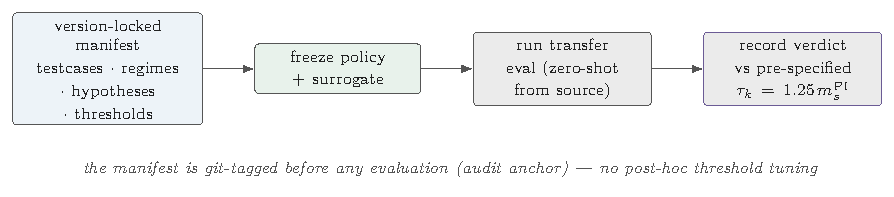
\includegraphics[width=0.97\linewidth]{fig_block3_protocol.pdf}
  \caption{Block 3 pre-specified transferability protocol. Controller-side transfer is tested against a testcase-specific PI threshold; surrogate-side transfer is tested by full Stage A/B/C recalibration on target telemetry.}
  \label{fig:protocol}

{\footnotesize\itshape Schematic; not derived from a dataset.}
\end{figure}

\begin{figure}[pos={!ht}]
  \centering
  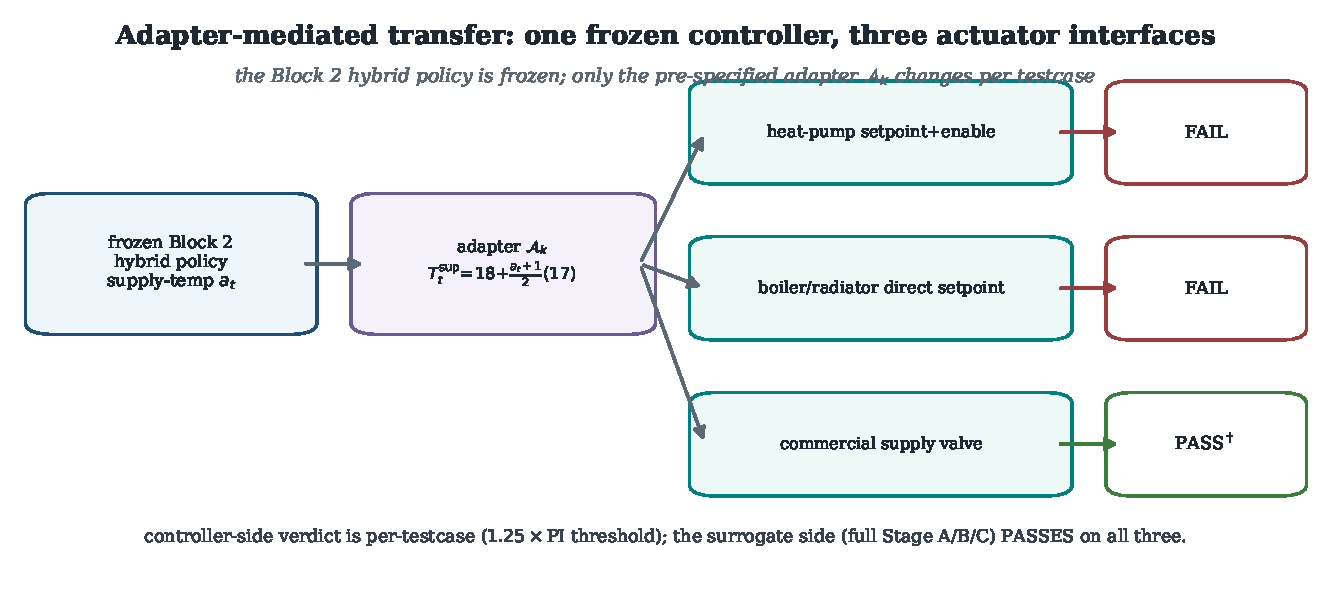
\includegraphics[width=0.97\linewidth]{fig_block3_adapter.pdf}
  \caption{Adapter-mediated transfer schematic. The frozen Block 2 hybrid policy is routed through a pre-specified actuator adapter $\mathcal{A}_k$ to each testcase's actuator interface; the controller-side verdict (against the $1.25\times$ PI threshold) is per-testcase, while full Stage A/B/C surrogate recalibration passes on all three.}
  \label{fig:adapter}

{\footnotesize\itshape Schematic; not derived from a dataset.}
\end{figure}

\begin{figure}[pos={!ht}]
  \centering
  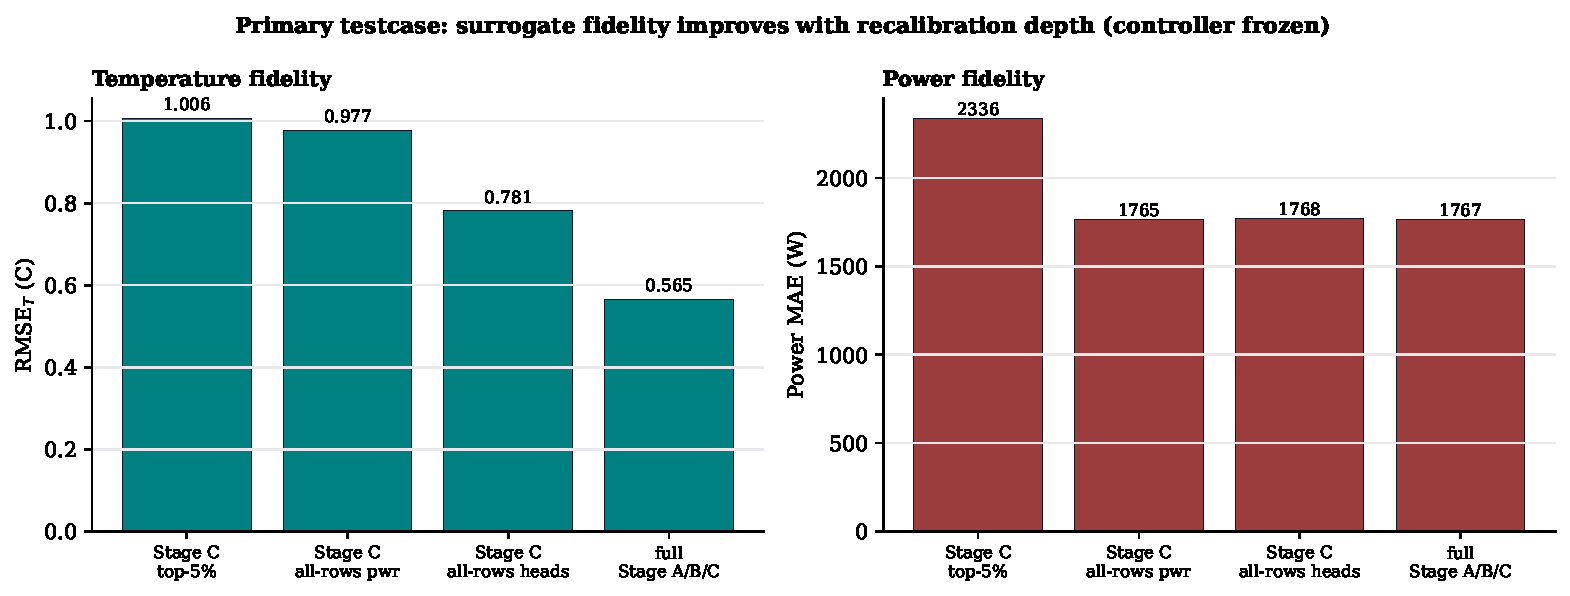
\includegraphics[width=0.92\linewidth]{fig_block3_regime_progression.pdf}
  \caption{Primary-testcase surrogate-fidelity progression across recalibration regimes. Temperature and power fidelity improve monotonically toward full Stage A/B/C, while the frozen controller's live $m_s$ is invariant by manifest scope.}
  \label{fig:regime_progression}

{\footnotesize\itshape Data: \texttt{reports/\allowbreak block3\_\allowbreak bestest\_\allowbreak hydronic\_\allowbreak heat\_\allowbreak pump\_\allowbreak transfer\_\allowbreak summary.csv}}
\end{figure}

\begin{figure}[pos={!ht}]
  \centering
  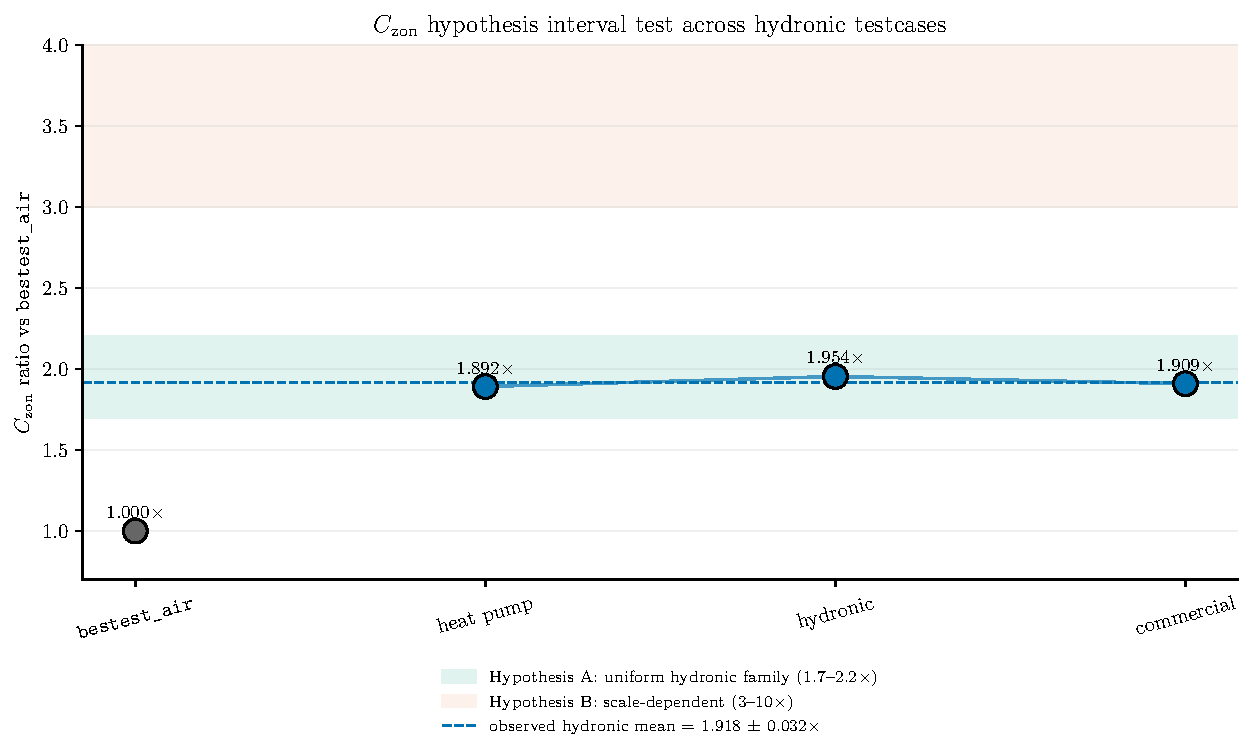
\includegraphics[width=0.82\linewidth]{final_eng_fig12_czon_hypothesis_interval.pdf}
  \caption{$C_{\mathrm{zon}}$ hypothesis-interval diagnostic. The observed ratios fall inside the uniform hydronic-family hypothesis A ($1.7$--$2.2\times$) and outside the scale-dependent hypothesis B ($3$--$10\times$).}
  \label{fig:czon_hypothesis}

{\footnotesize\itshape Data: \texttt{reports/\allowbreak block3\_\allowbreak transfer\_\allowbreak matrix.csv}}
\end{figure}

\begin{table}[pos={!ht}]
\centering
\small
\caption{Pre-specified target testcases and actuator adapters (manifest \texttt{testcase\_candidates}).}
\label{tab:testcases}
\begin{tabularx}{\linewidth}{l l >{\raggedright\arraybackslash}X l}
\toprule
Role & Testcase & Structural difference vs \texttt{bestest\_air} & Adapter \\
\midrule
Primary & \texttt{bestest\_hydronic\_heat\_pump} & hydronic loop driven by a heat pump & \texttt{hydronic\_t\_supply\_v1} \\
Secondary & \texttt{bestest\_hydronic} & boiler/radiator hydronic distribution & \texttt{hydronic\_direct\_supply\_v1} \\
Stretch & \texttt{singlezone\_commercial\_hydronic} & order-of-magnitude larger commercial zone + hydronic valve & \texttt{commercial\_hydronic\_valve\_v1} \\
\bottomrule
\end{tabularx}
\end{table}

\begin{table}[pos={!ht}]
\centering
\small
\caption{Per-testcase actuator-adapter mapping (verified from \texttt{configs/block3\_actuator\_mapping\_*.yaml}). All adapters share $h=\mathrm{clip}((T^{\mathrm{sup}}_t-18)/17,0,1)$; setpoint overrides are in kelvin.}
\label{tab:adapters}
\begin{tabularx}{\linewidth}{l l >{\raggedright\arraybackslash}p{40mm} >{\raggedright\arraybackslash}X}
\toprule
Testcase & Primary override & Override formula & Auxiliary overrides \\
\midrule
\texttt{heat\_pump} & \texttt{oveTSet\_u} (K) & $288.15+9h$ (zone setpoint $15$--$24^\circ$C) & \texttt{oveHeaPumY\_u}, \texttt{ovePum\_u}, \texttt{oveFan\_u} from $h$ \\
\texttt{hydronic} & \texttt{oveTSetSup\_u} (K) & $T^{\mathrm{sup}}_t+273.15$ (direct supply) & \texttt{ovePum\_u} from $h$; fixed comfort-band context \\
\texttt{commercial} & \texttt{dh\_oveTSupSetHea\_u} (K) & $T^{\mathrm{sup}}_t+273.15$ (district supply) & heating valves + pump from $h$; fixed zone/air context \\
\bottomrule
\end{tabularx}
\end{table}

\begin{table}[pos={!ht}]
\centering
\small
\caption{Pre-specified recalibration regimes. The controller is frozen in every regime.}
\label{tab:regimes}
\begin{tabular}{lll}
\toprule
Regime & Surrogate action & Controller action \\
\midrule
none & frozen \texttt{bestest\_air} surrogate recipe & frozen Block 2 hybrid controller \\
partial & Stage C residual-head recalibration only & frozen Block 2 hybrid controller \\
full & Stage A + Stage B + Stage C on target telemetry & frozen Block 2 hybrid controller \\
\bottomrule
\end{tabular}
\end{table}

\begin{table}[pos={!ht}]
\centering
\small
\caption{Primary-testcase per-regime detail. $m_s$ is invariant across rows because the controller is frozen by manifest scope; only surrogate fidelity changes (data: roadmap Section 15).}
\label{tab:primary}
\begin{tabularx}{\linewidth}{>{\raggedright\arraybackslash}p{42mm}rrr>{\raggedright\arraybackslash}X}
\toprule
Regime / artifact & RMSE$_T$ ($^\circ$C) & Power MAE (W) & $m_s^{\mathrm{RL}}$ & Status \\
\midrule
PI baseline (yearly) & -- & -- & 0.464 & reference \\
none: frozen controller & -- & -- & 0.665 & control FAIL \\
partial: Stage C top-5\% & 1.006 & 2336 & 0.665 & diagnostic \\
partial: all-rows power head & 0.977 & 1765 & 0.665 & diagnostic (power) \\
partial: all-rows heads & 0.781 & 1768 & 0.665 & surrogate cond.\ pass \\
full: Stage A/B/C & 0.565 & 1767 & 0.665 & surrogate PASS, ctrl FAIL \\
\bottomrule
\end{tabularx}
\end{table}

\begin{table}[pos={!ht}]
\centering
\small
\caption{Stretch-testcase pre-specified predictions versus observed outcomes (manifest \texttt{stretch\_testcase\_predictions}).}
\label{tab:predictions}
\begin{tabularx}{\linewidth}{>{\raggedright\arraybackslash}X l l l l}
\toprule
Prediction & Pre-reg.\ & A-priori & Observed & Verdict \\
\midrule
mode=none controller verdict & FAIL & 0.80 & threshold PASS & FALSIFIED \\
full surrogate RMSE gain & $[50,90]\%$ & 0.70 & 87.8\% & CONFIRMED \\
$C_{\mathrm{zon}}$ hyp.\ A (uniform) & $[1.7,2.2]\times$ & 0.35 & 1.91$\times$ & CONFIRMED \\
$C_{\mathrm{zon}}$ hyp.\ B (scale-dep.) & $[3,10]\times$ & 0.50 & 1.91$\times$ & FALSIFIED \\
$C_{\mathrm{zon}}$ hyp.\ C (failure) & non-convergence & 0.15 & converged (N=3) & FALSIFIED \\
\bottomrule
\end{tabularx}
\end{table}

\end{document}
